% options:
% thesis=B bachelor's thesis
% thesis=M master's thesis
% czech thesis in Czech language
% slovak thesis in Slovak language
% english thesis in English language
% hidelinks remove colour boxes around hyperlinks

\documentclass[thesis=B,czech,hidelinks]{FITthesis}[2012/06/26] %documentclass ... typ dokumentu (definovany v souboru .cls)

\usepackage[utf8]{inputenc} % LaTeX source encoded as UTF-8

\usepackage{graphicx} %graphics files inclusion
\usepackage{adjustbox}
\usepackage{multirow,tabularx}
\usepackage{xargs} 
\usepackage[pdftex,dvipsnames]{xcolor} 
\usepackage[colorinlistoftodos,prependcaption,textsize=tiny]{todonotes} 
% \usepackage{amsmath} %advanced maths
% \usepackage{amssymb} %additional math symbols

\usepackage{dirtree} %directory tree visualisation

% % list of acronyms
%\usepackage[acronym,nonumberlist,toc,numberedsection=autolabel]{glossaries}
%\iflanguage{czech}{\renewcommand*{\acronymname}{Seznam pou{\v z}it{\' y}ch zkratek}}{}
%\makeglossaries

\newcommand{\tg}{\mathop{\mathrm{tg}}} %cesky tangens
\newcommand{\cotg}{\mathop{\mathrm{cotg}}} %cesky cotangens
\newcommandx{\note}[2][1=]{\todo[linecolor=OliveGreen,backgroundcolor=OliveGreen!25,bordercolor=OliveGreen,#1]{#2}}
\newcommand{\code}[1]{\texttt{#1}}
\newcommand\tab[1][1cm]{\hspace*{#1}}

\department{Katedra softwarového inženýrství}
\title{Interaktivn{\' i} ovl{\' a}d{\' a}n{\' i} PC hry pomoc{\' i} chytr{\' e}ho telefonu}
\authorGN{Marek} 
\authorFN{Foltýn} 
\authorWithDegrees{Marek Foltýn} 
\supervisor{Ing. Filip K{\v r}ikava, Ph.D.}
\acknowledgements{Chtěl bych poděkovat vedoucímu práce Ing. Filipu K{\v r}ikavovi, Ph.D. za~pomoc a~p{\v r}íkladné vedení práce. Dále pak své manželce Veronice Foltýnové za~trpělivost a~ochotu vytvá{\v r}et prost{\v r}edí vhodné ke~tvorbě bakalářské práce, 
rodičům a~celé mé rodině za~velkou podporu ve~všech směrech. Děkuji také všem, kteří se podíleli na~testování hratelnosti hry.}
\abstractCS{Tato bakalářská práce se zabývá tvorbou systému pro~ovládání PC hry pomocí mobilního telefonu. Hlavním cílem je obohacení herního zážitku pomocí interaktivních prvků, které jsou na~mobilních telefonech k~dispozici. Součástí práce je analýza způsobů ovládání her, přehled interaktivních technologií v~mobilních telefonech a~samotná tvorba komunikačního systému, který je demonstrován na~jednoduché hře. }
\abstractEN{The main purpose of this thesis is to create an interactive PC game control system using smartphones in order to enhance the game experience. The thesis contains the analysis of different ways how a PC game can be controlled, the overwiev of interactive mobile technologies and also the communication system implementation, which is demonstrated in a simple game. }
\placeForDeclarationOfAuthenticity{V~Praze}
\declarationOfAuthenticityOption{1} %volba Prohlášení (číslo 1-6)
\keywordsCS{interaktivní ovládání PC hry, smartphone, komunikační systém, Cocos2d-x, RakNet}
\keywordsEN{interactive PC game controller, smartphone, communication system, Cocos2d-x, RakNet}

\begin{document} 

% \newacronym{CVUT}{{\v C}VUT}{{\v C}esk{\' e} vysok{\' e} u{\v c}en{\' i} technick{\' e} v Praze}
% \newacronym{FIT}{FIT}{Fakulta informa{\v c}n{\' i}ch technologi{\' i}}
\begin{introduction}
Videohry existují od~počátku prvních počítačů. \cite{rylich} Jejich možnosti se vyvíjejí podobně, jako se vyvíjí výpočetní a~grafický výkon, hardware a~další související technologie. Neustálé zmenšování součástek v~současné době nabízí vysoký výkon ve~velmi malých strojích: notebooky, chytré telefony a~dokonce i~hodinky s~vícejádrovými procesory. \cite{kupi}

Na~zmenšování hardwaru se adaptovaly také hry, které se v~hojné míře objevují i~na~přenosných zařízeních, jako jsou mobilní telefony, tablety a~další. Lidé tak~mohou hrát doslova kdekoli: nejen doma, ale~i~v~čekárně, ve~škole o~přestávce, na~cestě ve~vlaku a~podobně. Pokud si hráč chce zahrát, nemusí tak být doma, jako je tomu u~klasických počítačových a~konzolových her.

Mobilní zařízení jsou dnes velmi spojená s~lidmi a~jejich životem. Na~základě toho se nabízí otázka, zda~by tyto vlastnosti mohly nějakým způsobem obohatit herní interakci mezi lidmi. Existuje několik způsobů, které se o~tento cíl snaží:

Způsobem, jak~dosáhnout lepší mezilidské interakce ve~hře, je hra více hráčů: \textit{multiplayer}. Jedná se o~typ hry, kdy na~sebe v~herním světě reaguje více hráčů, ať už v~reálném čase, nebo pomocí sdílení pokroku ve~hře (např. žebříčky). Oba tyto způsoby sice zpřístupňují informace o~hře ostatních lidí, avšak ve~spojení s~internetem nemají až takový vliv na~mezilidskou komunikaci, spíše vylepšují vlasnosti herního světa, aby zlepšily hráčův zážitek. Jako příklad uvedu běžného hráče PC hry, který hraje doma v~pokoji multiplayerovou online hru přes~internet: Sice se pohybuje ve~stejném virtuálním světě jako další lidé, ale vliv na~mezilidskou komunikaci je minimální. Dalším příkladem je herní interakce pomocí sociálních sítí. Kromě svého pokroku ve~hře vidí hráč i~pokrok ostatních lidí a~někdy může ovlivnit jejich hru. Opět se ale nejedná o~sociální interakci ve~smyslu fyzické přítomnosti. Virtuální realita zde tvoří pouze prostor, skrz který ostatní hráči sledují jeden druhého.

I~přes~tyto nevýhody některých her existují způsoby, jak spojit virtuální realitu s~širší mezilidskou komunikací. Jedním z~nich je hra v~lokální síti, kdy jsou hráči fyzicky přítomni na~jednom místě (pokoj, garáž, …). Hráči prožívají stejný herní zážitek jako v~případě hry přes~internet, avšak umocněný přítomností ostatních hráčů. Reakce při~hře pak mohou obsahovat prvky komunikace typické pro mezilidský kontakt ve~fyzické přítomnosti: zvuk, vizuální a~fyzický kontakt, atd.

Další možností je hra na~jednom PC nebo konzoli. Pro~tento způsob je typické sdílení jedné obrazovky (monitor, televize) a případně ovládacích prvků (část klávesnice). Herní svět pak netvoří virtuální „bariéru“, přes kterou hráč vnímá ostatní lidi, ale stává se součástí prostředí společně s~lidmi, podobně jako například stolní hry.

\subsection{Cíl projektu}

Hraní na~sdílené obrazovce a~v~lokální síti se stalo hlavní motivací pro~tvorbu této práce. Přestože nejsem pravidelný hráč her, velmi mě zajímá využití her ve~snaze obohatit zážitek ze~společenské akce\footnote{Společenskou akcí je myšlena jakákoli vhodná příležitost trávení času s~více lidmi. Může to být například návštěva přátel, večírek nebo~volná hodina mezi vyučováním ve~škole.}. 

Jednou ze~způsobů, jak tohoto dosáhnout, může být využití mobilních telefonů. Dnešní mobilní telefony v~sobě obsahují velké množství prvků, které lze použít pro~interaktivní ovládání (dotykový displej, vibrace, zvuk, akcelerometr, gyroskop a~další senzory okolního prostředí), proto se jeví jako vhodné zařízení k~ovládání hry. Pokud spojíme multiplayerovou hru s~jednou hlavní obrazovkou (televize nebo monitor) a~ovládáním pomocí chytrého telefonu, vzniknou nové způsoby, jak propojit reálný svět s~hrou. Hráči mohou kromě klasického ovládání využít vlastní displej společně s~ostatními interaktivními prvky. Tím se herní pole rozšíří od~hlavní obrazovky na~další části prostoru.

V~této práci se budu zabývat hledáním způsobu, jak využít interaktivní prvky mobilních telefonů pro~ovládání počítačové hry. Smartphone tedy nebude sloužit jen jako samostatná herní konzole, ale ani jako simulace periferie typu myš nebo gamepad. Bude tvořit jednotný celek společně se~samostatným počítačem. Tuto myšlenku se budu snažit demonstrovat vytvořením systému komunikace mezi telefony a~počítačem a~jeho využitím v~jednoduché hře.

\end{introduction}

\chapter{Ovládání her}

V~první kapitole se budu nejprve zabývat problematikou ovládání her v~současné době a~to jak na~počítačích, tak i~na~dalších zařízeních. Stručně se zmíním o~historii vývoje ovladačů a~poté zmíním nejpoužívanější periferie v~dnešní době. Z~toto přehledu budu vycházet při zkoumání alternativních ovládacích prvků, jejich možností a přínosů.
 
Ovládání počítačových her úzce souvisí s~vývojem hardwaru a~především počítačových periferií. Nebudu se zabývat softwarovým návrhem uživatelského ovládání, ale spíše využitím hardwaru pro~herní účely. Hlavní náplní bude srovnání několika rozdílných způsobů ovládání, jejich přínosů a~nevýhod.

\section{Historie ovladačů}

Počítačové hry jako takové se začaly objevovat v~50. letech 20. století. Hardware dostupný v~této době nebyl určený pro~herní zaměření, např. známá hra \textit{Tennis for Two} vytvořená Williamem Higinbothamem v~roce 1958 v~národní laboratoři v~Brookhavenu využívala osciloskop jako grafický displej pro~zobrazení primitivní dvourozměrné hry a~jako ovládání sloužilo jedno tlačíko a~otočný regulátor.\cite{gamevshardware}

Větší rozvoj herního hardwaru začal v~roce 1971. Byl vytvořen první herní automat na~mince s~hrou \textit{Galaxy Game}. Jednalo se o~hru pro~dva hráče ovládánou jednoduchým joystickem. Později se začaly objevovat další automaty, využívaly jak tlačítka a~joystick, tak i~volant.

Hry se tedy objevovaly především na~herních konzolích. Vzhledem k~narustajícím prodejům osobních PC se hry dostávaly i~do~této oblasti, kde byla nejrozsířenejší periferií klávesnice. Vývoj herních konzolí se však nezastavil.

Převrat v~ovládání PC, a~to i~v~herním průmyslu, způsobil příchod počítačové myši, jak ji známe dnes. Mnoho herních konceptů bylo vylepšeno a~pro~hráče to představovalo větší pohodlí při~hraní. \cite{gamevshardware} Kromě toho se vyvíjely alternativní typy ovládání, některé úzce spojeny s~herním žánrem (joystick, volant), nebo naopak vhodné pro~velké množství her (gamepad).

Kromě klasických ovladačů se začaly objevovat také snahy o~přirozenější ovládání pomocí pohybu, tzv. \textit{motion sensing}. Vzniklo proto několik ovladačů a~herních konzolí, z~nichž nejvýznamější je Microsoft Kinect vzniklý v~roce 2010.\cite{wikicontrollers} Více se problematice ovládání pohybem věnuji v~sekci \ref{section:motion_capture}.

V~současné době se využívá široká škála způsobu a~technologií ovládání. Následující kapitoly budou věnovány těm nejvíce rozšířeným především v~osobních počítačích. Vysvětlím, k~čemu se dají vhodně využít a~jaké mají nedostatky. Následující přehled bude zároveň tvořit podklad pro~analýzu v~praktické části práce.

\section{Klávesnice}

Klávesnice je nejpoužívanější počítačovou periferií vůbec. Její princip je velmi jednoduchý: každé stisknutí či uvolnění tlačítka způsobí odeslání informace do~PC. Je možné detekovat události více tlačítek najednou, čehož využívají klávesové zkratky.

V~herním průmyslu se klávesnice využívá v~drtivé většině herních žánrů od~jednoduchých arkád, přes~závody až po~strategie. Jsou vhodné, pokud je potřeba rozlišit větší množství vstupů, které reprezentují jednotlivé klávesy.

Klávesnice ale nemusí být vždy ideální volbou. Diskrétní zpracování vstupu (stisknuto, nestisknuto) představuje nepohodlí při~ovládání závodní hry: v~zatáčení je zhoršená citlivost, auto buď zatáčí naplno, nebo vůbec. Tento nedostatek se vývojáři snaží řešit postupným natáčením kol, ale ani to není ideální. Při zatočení v~menší zatáčce je nutné přerušovaně uvolňovat klávesu, aby se vytvořila iluze mírně natočeného volantu. V~kombinaci s~myší může být nevýhodou horší dostupnost kláves vzdálenějších od~ruky.

\section{Myš}

Počítačová myš je druh polohovacího zařízení. Optický či laserový snímač detekuje pohyb myši po~podložce a~převádí jej na~pohyb kurzoru na obrazovce. Dále bývá myš vybavena několika ovládacími tlačítky.

Při~hraní má široké uplatnění tam, kde je využíván klasický kurzor nebo při~nutnosti souvislého, ale přesného pohybu jako například otáčení hráče v~FPS hře\footnote{First-person shooter - akční hra zobrazená z~pohledu herní postavy}.

Nevýhodou při~používání myši je jednostranná zátěž. Kvůli pohybu po~stole hráči zatěžují ruku s~myší více, než ruku na~klávesnici.

\section{Gamepad}

Gamepad je čistě herní periferie. Je to ovladač tvarovaný pro~použítí oběma rukama. Nachází se na~něm množství tlačítek a~může být doplněn jedním, nebo dvěma analogovými joysticky. Některé verze nabízejí i~vibrační odezvu. Nejdříve se využíval u~herních konzolí, s~rozvojem osobních PC se však stal i~zde velmi populární.

Primarní zaměření na~hry dělá z~gamepadu vynikající ovladač pro~mnoho herních žánrů. Eliminuje problém ergonomie myši a~klávesnice a~všechna tlačítka jsou snadno dostupná. Proto je velmi často využíván.

Z~hlediska intuitivního ovládání gamepad zaostává podobně jako myš a~klávesnice. Hry jsou s~ním sice dobře ovladatelné, avšak často je nutný trénink pro~zvládnutí složitějších principů ovládání a~tlačítkových kombinací.

\section{Joystick a volant}

Joystick a~volant představují ovladače pro~specifické druhy her.

Základní částí joysticku je páka umístěná kolmo v~pohyblivém kloubu. Má nejlepší uplatnění v~leteckých simulátorech, kde náklon páky mění polohu leteckých klapek. Ovládání je intuitivní a~snaží se přiblížit k~realitě.

Účelem volantu je simulace ovládání závodního vozu. Obvykle je dodáván s~dvěma nebo třemi pedály a~případně řadicí pákou. Vyšší modely mají vibrační odezvu, při vyjetí z~vozovky tak hráč cítí haptickou odezvu.

Joystick a~volant pomáhají věrně simulovat letecké nebo~závodní prostředí, pro~které jsou určeny. Na~rozdíl od~předešlých periferií jsou ale použitelné pouze v~úzké oblasti her, proto bývají nenáročnými hráči nahrazovány gamepadem nebo~klávesnicí.

\section{Dotyková obrazovka}

Dotyková obrazovka na~osobních počítačích není v~současné době masově využívána. Větší rozšíření má v~oblasti mobilních zařízení, jako jsou mobilní telefony a~tablety, proto se více problematice dotykové obrazovky budu věnovat v~sekci \ref{section:touchscreen}. Některé hry však využívají dotykovou obrazovku jako~náhradu za~jiné periferie (např. myš). Záleží pak na~návrhu samotné hry, zda toto ovládání přinese nějaké benefity, či~bude spíše překážkou.

\section{Ovládání pohybem}

Kromě tradičních hardwarových periferií existují další technologie, jak~ovládat hry, a~to~pomocí přirozeného pohybu člověka. Tyto systémy snímají gesta a~pohyby hráče nebo ovladače a~podle nich vypočítají reakci ve~hře. Ovládání bývá snadné na~naučení, protože navozuje pocit přirozené reakce na~podněty herního prostředí.

V~této kapitole zmíním dvě technologie: motion capture (neboli snímání pohybu těla) a~ovládání pomocí akcelerometru. Obě tyto technologie rozšiřují možnosti interakce s~elektronickými zařízeními, jsou včak odlišně složité a~fungují na~jiném principu.

\subsection{Akcelerometr}
\label{section:accelerometer}

Akcelerometr je elektromechanická součástka, která měří zrychlení sil ve~3 osách. Tyto síly mohou být statické, jako například tíhová síla, nebo dynamické - způsobeny pohybem nebo vibrováním akcelerometru.\cite{acc} Tato součástka umožňuje detekovat natočení zařízení v~prostoru a~jeho přibližný pohyb.

V~herním průmyslu se využívá především v~mobilních zařízeních a~v~herních konzolích. Může nahradit joystick, emulace volantu nebo polohovacího zařízení. 

V~případě, že~jako vstupní zdroj informace je poloha zařízení, může v~nevhodném prostředí docházet k~rušení: například při~jízdě v~autobuse je téměř nemožné hrát závodní hru, jelikož při zatáčení autobusu je síla působící na~akcelerometr vychýlená a~dochází k~nechtěnému zatáčení.

Další informace o~pohybovém senzoru jsou uvedeny v~sekci \ref{section:accelerometer}.

\subsection{Motion capture}
\label{section:motion_capture}

Velmi zajímavou technologií je ovládání pohybem, tzv. \textit{motion capture}. Jedná se o~snímání části nebo~celého těla a~jeho převod v~reálném čase na~digitální model. Ten se využívá mimo jiné k~ovládání hry. Nejvýraznějším ovladačem v~herním průmyslu se stal \textit{Kinect} vyvinutý v~roce 2009 firmou Microsoft. \cite{meetthekinect}

Motion capture se hodí například pro~sportovní nebo~akční hry a~to i~při více hráčích. Nevýhodou může být nutnost poměrně velkého prostoru pro~potřeby hraní.

\section{Srovnání}

V~minulých kapitolách jsem stručně popsal několik způsobů, jakým lze ovládat hry. Každý znich má řadu výhod i~nevýhod. Následující tabulka obsahuje shrnutí těchto ovladačů a~porovnání jejich možností. Vzhledem k~tématu této práce se~zde budu zabývat především tím, jak je daný způsob interaktivní a~zda tak může obohatit zážitek ze~hry.

\begin{table}[h]
\caption{Srovnání herních ovladačů}
\begin{tabularx}{\textwidth}{|l|X|X|}
\hline
\textbf{Ovladač} & \textbf{Výhody} & \textbf{Nevýhody} \\ \hline
Klávesnice & - počet kláves \newline - široké využití & - pouze dva stavy tlačítka (stisknuto, nestisknuto) \newline - některé klávesy hůře dostupné \\ \hline
Myš & - přenost & - jednostranná zátěž \\ \hline
Gamepad & - ergonomický \newline - navržen pouze pro~hry \newline - interaktivní vibrační odezva & - ovládání není intuitivní, je třeba se jej naučit \\ \hline
Joystick, volant & - věrně simuluje realitu \newline - interaktivní vibrační odezva & - vhodné jen pro~některé herní žánry \\ \hline
Dotyková obrazovka & - široké využití \newline - provázanost grafiky s~ovládáním & - v~některých hrách neúspěšně simuluje jiné periferie \\ \hline
Akcelerometr & - intuitivní & - rušení např. v~dopravním prostředku či~jiném pohybu \\ \hline
Motion capture & - velmi přirozené ovládání & - potřeba většího prostoru \\ \hline

\end{tabularx}
\end{table}


\chapter{Interaktivní prvky v~mobilních telefonech}

V~první kapitole jsem představil nejběžnější herní ovladače, které využívají herní konzole a~osobní počítače. V~následující kapitole se budu věnovat analýze mobilních telefonů a~jejich senzorů interagujících s~okolním prostředím. Popíšuc jejich princip fungování a~budu zkoumat herní využití jak v~mobilních hrách, tak jako interaktivní ovladač pro~počítačovou hru. Některé z~těchto senzorů pak využiji při~tvorbě interaktivního ovladače v~kapitole~\ref{chapter:implementation}.

Senzory se budu snažit využít tak, aby mobilní telefon nesloužil pouze jako vstupní zařízení, ale byl provázán s~hrou samotnou. To umožní rozšířit herní realitu a ovladač vytvoří neoddělitelný celek s~hrou. Zároveň to nabídne nové možnosti herních principů, které by na~tradičních periferiích nebyly realizovatelné.

\section{Dotykový displej}
\label{section:touchscreen}

Dotykový displej je označení pro~kombinaci zobrazovacího displeje a~průhledné vrstvy schopné zaznamenávat dotyky vnějších těles, obvykle prstu nebo~stylusu. Existuje několik technologií snímání dotyku, stručně popíšu pouze nejrozšířenejší technologi v~dnešních mobilních zařízeních: kapacitní dotykový panel.

Kapacitní dotykový panel využívá elektrické vodivosti vnějších těles. Dotyk takového tělesa s~povrchem displeje naruší elektrostatické pole obrazovky a~jeho lokaci pak dále zpracuje řadič. Proto kapacitní displeje fungují pouze s~vodivými předměty jako je lidský prst nebo~speciální stylus. \cite{gray2013does}

Dotykové displeje nabízejí velmi široké možnosti uplatnění ve~hrách. Na~rozdíl od~klasických ovladačů totiž propojují zobrazení grafiky se~samotným ovládáním. Například přesun objektů v~herním světě je velmi přirozený: hráč se jednoduše dotkne objektu a~tahem prstu jej přesune po~obrazovce. Ve~srovnání s~počítačovou myší odpadá \textit{mezivrstva} ve~formě periferie připojené k~zařízení a~hráčův prst se tak stává samotným kurzorem.

Možnosti dotykových displejů, jako jsou gesta a~snímání více dotyků najednou, zásadním způsobem zjednodušují ovládání mobilních telefonů a~tedy i~mobilních her. Některé jsou přímo postaveny na~využití dotykových displejů, např. úspěšná hra \textit{Fruit Ninja}\cite{fruitninja}. Hlavní ovládací prvek tvoří tah prstem, který simuluje seknutí čepelí. Hráč se snaží prstem přeseknout co největší množství letícího ovoce najednou. Hra se stala příkladnou ukázkou využití dotykové obrazovky: letící ovoce je podnětem, abyse hráč trefil do~daného místa na~obrazovce a ovládání přímo koresponduje se zobrazovanou grafikou (pokaždé je pro~optimální přeseknutí potřeba jiné gesto prstem). Hra a~ovládání tak splývají v~jednu ucelenou část.

\begin{figure}
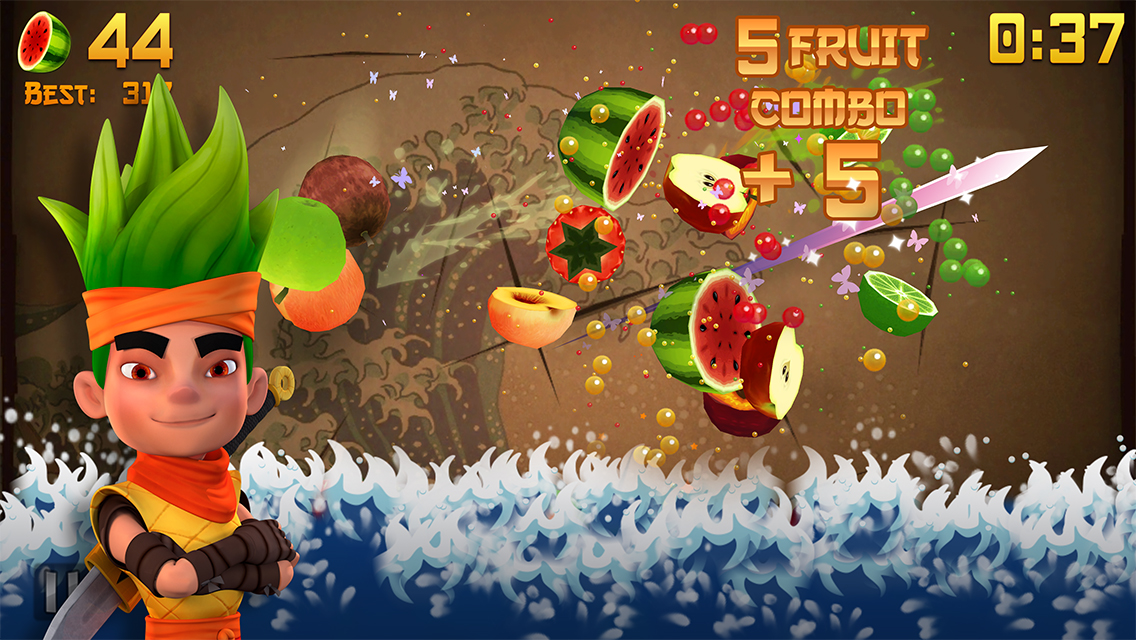
\includegraphics[width=\textwidth]{fruit_ninja}
\caption{Využití dotykové obrazovky ve hře Fruit ninja\cite{fruitninja}}
\end{figure}

Této provázanosti se dá využít i~v~počítačové hře ovládané mobilním telefonem: Hlavní herní scéna je zobrazována na~displeji počítače a~hráč drží v~ruce ovladač (mobilní telefon), který je úzce provázán s~hrou v~PC. Dotyková obrazovka pak plní funkci jak ovládací, tak i~zobrazovací. To nemusí být nutně výhodou, protože při ovládání hry se hráč přirozeně soustředí především na~herní obraz v~PC a~může být nepohodlné často měnit pohled z~monitoru na~mobil. Pokud je ale hra pro více hráčů, otevírají se nové možnosti, jak využít individuální obrazovku pro~každého hráče, který tím získá soukromý zobrazovací prostor a~ten může poskytovat přídavné informace. Tuto techniku využívám v~implementaci demonstrační hry, kdy hráč při získání bonusu neviditelnosti zmizí z~hřiště na~hlavní obrazovce a~začne se mu na~mobilním displeji zobrazovat kompletní herní scéna i~se~zmizelým hráčem. Protivníci tím pádem ztrácí informaci o~hráčově pozici a~on získává herní výhodu. Této techniky lze dosáhnout pouze úzkým provázáním hry a~ovladače. Vzhledem k~těmto schopnostem mobilních telefonů v~kombinaci s~dostatečným výkonem, dalšími senzory a~rychlou bezdrátovou komunikací má využití dotykového displeje velký potenciál.

Kromě toho je dotyková obrazovka v~implementaci využita jako vstupní zařízení ve~formě tlačítek a~to jak při~klasickém ovládání, tak i~při~aktivní neviditelnosti souběžně se~zobrazováním hry.

\section{Akcelerometr}
\label{section:accelerometer}

Dalším interaktivním senzorem akcelerometr, jehož princip vysvětluje kapitola \ref{section:accelerometer}. Objevuje se jak v~ovladačích k~herním konzolím, tak v~mobilních telefonech, kde plní různé funkce: zajišťuje automatickou orientaci displeje v~závislosti na~natočení mobilu, pohybová gesta jako například zatřesení~nebo položení displejem dolů mohou sloužit k~ovládání systému a~široké využití má ve~hrách.

Existuje velké množství mobilních her využívající náklon telefonu k~ovládání. Následující výčet obsahuje přehled nejčastějších použití ve~hrách a~související příklady \cite{accelerometergames}:

\begin{itemize}
	\item Simulace volantu v~závodní hře (Lane Splitter, Jet Car Stunts)
	\item Náklon telefonu odpovídá náklonu herní podložky (Crazy Labyrinth 3D)
	\item Využití akcelerometru jako joysticku v~leteckém simulátoru (Skies of Glory)
	\item Náklon telefonu mění pozici herního objektu (Donkey Jump, Box Busters)
\end{itemize}

Pro~interaktivní ovladač k~PC hře je použití akcelerometru ideální příležitostí. Pohyb herního objektu náklonem telefonu je pro~člověka přirozenější a~vtahuje hráče intenzivnějši než~ovládání tlačítky. 

Využití akcelerometru v~praktické části práce je podobné jako ve~hře Donkey Jump, na~rozdíl od~ní však nabídne pohyb do~všech směrů ve~2D prostoru.

\section{Gyroskop}

Gyroskop je součástka pro~detekci polohy zařízení. Měří změnu úhlu natočení telefonu kolem své osy. To umožňuje detekovat pohyb zařízení lépe než~akcelerometr, ale vzhledem k~detekci relativní změny se postupem času objevuje odchylka a~proto se gyroskop využívá v~kombinaci s~akcelerometrem a~někdy též s~kompasem. Díky tomu je možné určit natočení telefonu vůči gravitační síle a~detekovat změnu polohy zařízení ve~všech směrech. \cite{gyroscope}

\section{Senzor přiblížení}

Senzor přiblížení, nebo také \textit{proximity senzor} funguje na~principu detekce elektromagnetického záření, které generuje vysílač. V~případě přiblížení objektu do~blízkosti snímače je zaznamenán odraz záření zpět k~senzoru a~je tak vyhodnocena vzdálenost objektu. \cite{proximity}

Nejběžnější využití proximity senzoru v~mobilním telefonu je při~hovoru. Před~přiložením k~uchu senzor detekuje blízkost hlavy a~zhasne displej. Zabráním tím tak nechtěnému ukončení hovoru dotykem ucha s~obrazovkou.

Herní využití proximity senzoru není rozšířené, neexistují žádné hry interaktivně využívající proximity senzor ve~hře, pouze simulace tlačítka v~PC hře podomácku vyrobeným senzorem přiblížení. \cite{proximitygame}

\section{Ostatní senzory}

Současné mobilní telefony mohou disponovat ještě několika dalšími senzory okolního prostředí, ale vzhledem k~minimálnímu využití v~herní oblasti zde nebudou více zkoumány. Jedná se například o~senzor okolního světla, teploměr a~magnetický senzor. 

\section{Shrnutí}

V~této kapitole byly popsány nejčastější interaktivní senzory vyskytující se v~dnešních mobilních telefonech, jejich princip a~možné využití. V~kapitole \ref{chapter:implementation} se budu snažit některé z~nich využít při~tvorbě interaktivního ovladače pro~PC hru. 

\chapter{Podobná řešení}

Před samotnou tvorbou softwarového projektu zmíním podobné systémy na~trhu. V~současné době již existují řešení využívajíci mobilní telefon k~ovládání jiné hry. Každé z~nich však obsahuje nedostatky a~narušuje tak výslednou interaktivitu hry.

\section{Telefon jako univerzální gamepad}

Na~internetu existuje velké množství aplikací, které nabízejí funkcionalitu podobnou bezdrátovému gamepadu. Ukázkou takové aplikace je např. Mobile Gamepad \cite{mobilegamepad} Po~nainstalování příslušného ovladače do~PC je možné využít telefon jako vstupní zařízení: umožňuje nastavit si tlačítka na~displeji, pohybový senzor jako joystick atd.

Výhodou tohoto řešení je možnost ovládat PC podobně jako jiné ovládací periferie a~díky tomu není ovladač vázán na~konkrétní hru. Co však brání použití v~interaktivní hře, je absence jiných funkcí než těch, které již obsahují gamepady a~podobné ovládací prvky. To je způsobeno univerzálností ovladače. Pro~zachování standardizovaného ovládacího rozhraní a~chování jako klasické vstupní zařízení počítače není umožněna širší komunikace s~hrou. Tyto aplikace tak nabízejí stejnou nebo často i~méně kvalitnější alternativu ke~klasickým herním gamepadům a~jiným ovladačům. 

\todo{obrázek univerzálního gamepadu}

\section{Apple AirPlay}

Společnost Apple nabízí pro~své telefony funkci sdílení obrazu na~externí obrazovku. Toho je docíleno pomocí zařízení AppleTV a~bezdrátové technologie AirPlay\cite{airplay}.

Toto řešení již lépe využívá interaktivní možnosti mobilních přístrojů, integrovaný displej tvoří druhou obrazovku, může zobrazovat ovládání dobře optimalizované pro~konkrétní hru nebo~dodatečné informace o~hře (skóre, počet ujetých kol atd.). Zásadní nevýhodou však je nemožnost hrát hru ve~více hráčích kvůli zvolené architektuře: herní logika včetně vykreslování běží na~straně mobilního zařízení a~do~externí obrazovky se přenáší pouze obraz.

\todo{obrázek AirPlay}

\section{AirConsole}

Řešením, které se nejvíce podobá tématu této bakalářské práce, je herní platforma švýcarského startupu AirConsole\cite{airconsole}. Jedná se o~webovou aplikaci společně s~multiplatformní mobilní aplikací. Pomocí webového prohlížeče se vytvoří hra a~k~ní se připojí telefony jako ovladače. V~nabídce je několik různých her a~každá má vlastní ovladač v~rámci mobilní aplikace. Samotná hra tedy probíhá na obrazovce počítače. AirConsole také poskytuje API, takže lze vytvořit vlastní hru v~HTML5 nebo herním enginu Unity a~propojit ji~s~tímto systémem.

Bohužel i~zde se objevují nedostatky. Spojení probíhá přes externí servery, konkrétně přes infrastrukturu Google\cite{airconsole}. Kvůli nutnosti komunikace \textit{PC - Google server} a \textit{telefony - Google server} má spojení vyšší odezvu, což silně ovlivňuje zážitek ze~hry. Ovládací rozhraní je vytvořené pomocí HTML5, na~displeji se tedy vykresluje webová vrstva. Zpracování dotyku v~tomto případě není ideální, objevují se chyby (například špatná detekce kliknutí) a~projevuje se vyšší odezva. Zároveň ovládání nevyužívá interaktivní možností mobilních telefonů, jediný možný způsob interakce je pomocí dotykového displeje. AirConsole tak vytváří podobnou funkcionalitu, jako je emulace gamepadu.

Přes~všechny tyto nedostatky se AirConsole nejvíce blíží projektu této bakalářské práce, především hlavním cílem, a~to vytvořit herní platformu podporující mezilidskou komunikaci lidí fyzicky přítomných na jednom místě.

\todo{obrázek AirConsole}

\section{Možnosti řešení}

V~rámci bakalářské práce jsem nalezl tři možnosti řešení, jak odstranit nedostatky předchozích systémů:

\subsection{Rozšíření existující PC hry}

Prvním způsobem vytvoření ovládání pomocí mobilního telefonu je vytoření mobilního ovladače k~již existující PC hře s~otevřeným zdrojovým kódem. Stěžejní částí by bylo vytvoření „adaptéru“ napojeného na~mobilní telefon. Nevýhodou je rozsáhlost takového projektu a~složitost jejího rozšíření o~interaktivní prvky.

\subsection{Univerzální herní ovladač}

Druhým způsobem je vytvoření mobilní aplikace poskytující rozhraní pro~komunikaci s~libovolnou hrou. Takto je vytvořen systém AirConsole. Jeho velkou výhodou je univerzálnost použítí, kdy jedna mobilní aplikace může být využita pro~mnoho her, které implemetují požadované rozhraní. Pro~univerzální použití včetně interaktivních senzorů by však muselo rozhraní podporovat velké množství funkcí, např. definice ovládání, načtení grafiky z~libovolné hry, poskytnutí ovládací logiky mobilnímu ovladači a~funkce pro~využití mobilních senzorů. Složitost tohoto řešení však překračuje rozsah bakalářské práce.

\subsection{Komunikační modul}

Třetí možností je vytvoření systému pro~síťovou komunikaci PC~a ovladače. Takovéto řešení by bylo možné použít v~libovolné hře, ale~s~nutností vytvořit mobilní ovladač na~míru ke~hře. Není třeba vytvářet rozhraní pro~sdílení herní logiky a~grafických prvků, neboť to může být implementováno v~ovladači nebo~vyřešeno sdílením zdrojového kódu s~hrou. Zařízení si budou mezi~sebou posílat zprávy s~herními informacemi, na~které budou obě zařízení reagovat definovaným způsobem. Tento návrh umožňuje vytvořit snadno integrovatelný systém komunikace nezávislý na~konkrétní hře. Mobilní zařízení budou mít zároveň širší možnosti využití hardwaru. Tento systém jsem zvolil jako~implemetaci v~bakalářské práci, protože eliminuje nevýhody stávajících řešení a~zároveň nabízí přijatelný kompromis mezi složitostí a~univerzálností pro~případ použití v~dalších hrách. 

\chapter{Tvorba systému}
\label{chapter:implementation}

Informace o~možnostech ovládání hry pomocí mobilního telefonu v~následující kapitole využiji v~praxi a~vytvořím systém, ve~kterém bude mobilní telefon v~roli interaktivního ovladače PC hry. To vyžaduje tvorbu komunikačního protokolu a~jeho implementaci ve~hře. Softwarový projekt komunikačního protokolu i~hry samotné je hlavní náplní praktické části mé bakalářské práce.

Struktura kapitoly odpovídá vývojovým fázím softwarového projektu. \cite{si} První část je zaměřena na~analýzu systému, požadavky a~softwarový návrh, v~implementační fázi zmíním některé zásadní části realizace, testování programu a~hratelnosti a~na~závěr se budu zabývat možnostmi, jak by bylo možné vytvořený systém rozšířit v~budoucnosti.

\section{Požadavky}

Cílem první fáze softwarového projektu je specifikace vlastností projektu. Určení prostředí, ve kterém bude systém nasazen a vymezení funkcionalit nutných pro naplnění účelu systému.

Pro ucelený přehled o~systému nejprve popíšu běžný průběh hraní hry postavené na systému vytvořeném v~této práci:

Skupina hráčů s~chytrými telefony se připojí do jedné WiFi sítě společně s~PC, kde poběží hra (server). Poté spustí ovladač v~mobilním telefonu, který automaticky vyhledá hry dostupné v~lokální síti. Po kliknutí na název nalezené hry naváže ovladač spojení s~hrou. Hráč, který může měnit nastavení hry (administrátor, typicky první připojený hráč), nastaví parametry hry a po připojení všech hráčů zahájí hru. V~případě odpojení nebo ztráty spojení bude možné se do hry opět připojit. Po skončení hry se systém dostane do stejné fáze jako před jejím zahájením, tj. bude opět možné měnit herní parametry apod.

Z~výše uvedeného scénáře budu vycházet při tvorbě požadavků, které jsem rozdělil do dvou částí: komunikační protokol a~hra samotná. Každá část má vlastní seznam funkčních a~nefunkčních požadavků. Tyto požadavky představují základní kritéria pro~návrh architektury systému a~jeho funkcionalit.

\subsection{Komunikační protokol}

Účelem komunikačního protokolu je v~tomto případě zajistit obousměrnou výměnu zpráv mezi mobilním telefonem (dále jen \textit{ovladačem}) a počítačem (dále jen \textit{hrou}). K~tomu je vhodné použít stejný systém v~obou zařízeních, aby bylo možné implementovat komunikační systém pouze jednou a ne na každou platformu zvlášť. Stejně tak je třeba zachovat identickou definici síťových zpráv mezi všemi zařízeními.

Ovladače budou s~hrou komunikovat v~lokální WiFi síti. Při návrhu protokolu tak musíme brát v~potaz nedostatky technologie, v~tomto případě především spolehlivost spojení. Při bezdrátové komunikaci je nutné počítat s~výpadky signálu. Může je způsobovat nedostatečný výkon WiFi routeru, příliš velká vzdálenost od vysílače nebo objekty v~prostoru, které brání šíření signálu. Proto je třeba u~zpráv rozlišit, zda je nutné, aby byla doručena spolehlivě (např. kliknutí hráče na tlačítko), nebo zda systému nevadí případná ztráta zprávy (např. často se opakující informace z~pohybového senzoru,). 

Vzhledem k~univerzálnímu zaměření systému je vhodné oddělit přenos zpráv a jejich zpracování (parsování) pro dosažení větší modularity. Dále je výhodné umožnit  konfiguraci síťových parametrů, a odpovídala požadavkům konkrétní hry.

Specifikace funkčních požadavků softwarového systému popisuje základní chování systému a jeho dílčích částí. Tato specifikace slouží jako nutný základ při návrhu projektu a také jako podklad pro zhodnocení úspěšnosti aplikace. \cite{pozadavky}

Pro komunikační protokol platí tedy následující funkční požadavky:

\begin{enumerate}
	\item Musí být možné nalézt všechny běžící hry v~lokální síti.
	\item Každá síťová zpráva má tyto vlastnosti: typ zprávy, data zprávy, spolehlivost doručení, zachování pořadí.
	\item Hra i ovladač dokáží detekovat ztrátu spojení.
	\item Síťový port (nebo jejich rozsah) a další lze definovat zvlášť jak pro ovladač, tak pro hru.
	\item Ovladač umožňuje odeslání informací o~interakci uživatele (kliknutí na tlačítko, data z~pohybového senzoru)
	\item Ovladač je schopen přijímat informace o~stavu hry (herní události, kompletní stav hry pro vykreslení na mobilním displeji)
\end{enumerate}

Funkční požadavky jsou doplněny požadavky nefunkčními, které specifikují kvalitu aplikace podle kritérií, mezi která se řadí například výkon, splolehlivost, rozšiřitelnost a další. Zaměřil jsem se především na cílovou platformu, rozšiřitelnost a modulárnost pro jednoduché nasazení v~dalších hrách:

\begin{enumerate}
	\item Síťová komunikace probíhá v~rámci stejné WiFi sítě. Podpora pro bluetooth a další technologie není implementována.
	\item Komunikační systém běží na alespoň jedné mobilní platformě (Android, iOS nebo Windows Phone) a alespoň jedné PC platformě (Windows, Linux nebo OS X).
	\item Systém je modulární: je možné definovat vlastní typy zpráv, jejich strukturu a vlastnosti podle požadavků hry.
	\item Parsování zpráv nezávisí na komunikačním frameworku. Je možné implementovat rozdílné parsování nebo i několik různých metodik najednou.
	\item Zdrojový kód komunikačního modulu je sdílený mezi hrou a ovladačem.
	\item Komunikační modul nezávisí na herním engine a tím pádem je využitelný v~libovolné jiné hře.
\end{enumerate}

\subsection{Hra}

Požadavky na hru samotnou se v~první řadě netýkají herního žánru a obsahu, ale snaží se především využít komunikační systém a možnosti interaktivity. Volba žánru a konkrétního typu hry je proto přesunuta až do fáze návrhu, kde bude nutné vhodně navrhnout zapracování interaktivních prvků do herních mechanik.

Důležitou vlastností hry je demonstrace nových možností oproti klasickým ovladačům. Mezi ně se mimo jiné řadí schopnost vykreslování grafiky v~mobilní obrazovce. Tuto a další nové možnosti je třeba ve hře 
výrazně prezentovat.

Pro celou hru (ovladač i PC) platí následující funkční požadavky:

\begin{enumerate}
	\item Hra využívá k~ovládání pohybový senzor mobilního telefonu a dotykovou obrazovku.
	\item Ovladač je schopen vykreslit herní scénu nebo její část na~obrazovce mobilního telefonu.
	\item Hra je určena pro 2 až 8 hráčů (ovladačů).
	\item Mobilní telefon může využívat vibrace jako interaktivní odezvu na~události ve hře.
 	\item Každá instance hry může mít nastaven název serveru a herní parametry.
	\item Parametry hry může měnit právě jeden z~připojených hráčů.
	\item Zvolený herní žánr je vhodný pro hru více hráčů a obsahuje jak kooperativní, tak kompetitivní složku.
	\item Veškerá konfigurace hry probíhá pomocí ovladače: po spuštění hry na PC již není potřeba další obsluha PC (mimo ukončení hry).
	\item Zobrazováním hry nebo její části na displeji mobilního telefonu přináší danému hráči taktickou výhodu oproti ostatním.

\end{enumerate}

Nefunkční požadavky na hru zahrnují především použití cílové platformy:

\begin{enumerate}
	\item Ovladač poběží na alespoň jedné mobilní platformě (Android, iOS nebo Windows Phone).
	\item Hra poběží alespoň na jedné PC platformě (Windows, Linux nebo OS~X).
	\item Použitý herní engine je multiplatformní a použitelný jak ve hře, tak v~ovladači.
\end{enumerate}

\section{Návrh}

Návrh systému je druhou fází softwarového projektu. Obsahuje podrobnější popis komponent systému, jejich objektů a popis jejich vzájemných vztahů.

Hra pro PC i ovladač používají dvě základní komponenty. První z~nich je síťový modul zajišťující veškerou síťovou komunikaci a druhou komponentou je herní engine. 

\subsection{Komunikační modul}

Úkolem komunikačního modulu je zajistit výměnu zpráv v~lokální síti. Kromě toho definuje obecnou síťovou zprávu a její vlastnosti. Modul tedy tvoří dvě základní komponenty: \textit{Box} a \textit{Connector}. 

Hlavním přínosem modulu je odstínění implementace síťové vrstvy od hry a herního enginu a velmi snadné nasazení v~libovolné jiné hře zaměřené nejen na interaktivní ovládání pomocí mobilního telefonu. Výhodou vytvoření abstraktní vrstvy v~porovnání s~přímým použitím RakNetu je především zjednodušení navázání spojení, manipulace s~dakovými pakety (Boxy) a nezávislost na vnitřní implementaci.

\todo{obrázek tříd Connector a Box}

\subsubsection{Box}

\textit{Box} je objekt reprezentující síťovou zprávu. Jeho cílem je zapouzdřit veškeré informace potřebné pro práci se síťovou zprávou Používá se při obou směrech komunikace, což znamená, že se vytváří před odesláním, ale také po přijetí zprávy.

Obsahuje data zprávy, typ zprávy, adresu příjemce (pokud bude zpráva odeslána), nebo adresu odesílatele (pokud byla zpráva přijata), dále vlastnosti doručení, mezi které patří spolehlivost (spolehlivé doručení znamená, že odesílající zařízení čeká na potvrzení přijetí zprávy), priorita, jak rychle má být zpráva doručena (zprávy s~nízkou prioritou mohou být řazeny do fronty a odeslány najednou, což šetří síťový provoz), nebo nastavení, zda je nutné dbát na zachování pořadí zpráv, v~jakém byly odeslány.

\subsubsection{Connector}

\textit{Connector} je objekt, který stanovuje programové rozhraní veškerého fungování síťové komunikace: obsahuje metody pro aktivování síťových rozhraní, připojování a odpojování klientů, posílání a příjem \textit{Boxů}. 

\subsubsection{RakNet}

Hlavičková definice \textit{Connectoru} i \textit{Boxu} tvoří abstraktní rozhraní nad samotnou implementací a umožňuje tak snadnou změnu platformy, případně síťové knihovny. Pro implementaci rozhraní jsem zvolil knihovnu RakNet.

RakNet je multiplatformní síťová se zaměřením na hry napsaná v~C++. Vyznačuje se velmi nízkými nároky na hardware, kvalitní dokumentací a množstvím funkcionalit, které se často využívají v~multiplayerových hrách. \cite{raknet} Mezi ně patří například Lobby systém\footnote{Lobby systém - virtální místnost, kde se shromažďují hráči před začátkem online hry. Obvykle nabízí chat mezi hráči, volbu herních místností nebo žebříček výsledků.}, šifrování komunikace nebo peer-to-peer spojení mezi hráči. Veškerá komunikace je postavena na protokole UDP, přesto knihovna obsahuje podporu pro spolehlivé doručení zpráv.

Knihovnu jsem zvolil především pro její snadné použití a podporu jak klasických počítačů i mobilních platforem. Stejnou implementaci modulu je tak možné využít v~ovladači i ve hře na PC.

\subsection{Hra}

Návrh hry se skládá z~několika částí. Prvním krokem je volba herního žánru. Poté se budu věnovat hledání herního enginu, na kterém bude hra postavena. Poslední částí bude již samotný návrh struktury systému, objektů, vztahů mezi nimi a tvorba samotného komunikačního protokolu.

\subsubsection{Volba herního žánru}

Jak bylo zmíněno v~analýze, důležitým požadavkem pro hru je možnost efektního využití interaktivních možností chytrých telefonů. K~tomu musí být uzpůsobem herní žánr tvořící kostru veškeré hratelnosti. Proto jsem nejprve zvolil dva směry a porovnával jejich výhody a nevýhody:

Prvním z~nich je akční 2D hra, kde kamera zobrazuje scénu zhora. Hlavním pilířem hry je souboj dvou týmm a cílem je dosáhnout většího počtu zásahů, než protivník. Každý hráč by ovládal jednu postavu vybavenou zbraní. Mezi interaktivní prvky lze zařadit ovládání postavy pohybovým senzorem a intuitivní míření pomocí dotykového displeje (místo dotyku prstu a střed obrazovky vytvoří přímku definující směr výstřelu). Inovativní by mohlo obsahovat zobrazení herní mapy: hlavní herní území se zobrazuje na obrazovce, kterou vidí všichni hráči. Mohou se tam ale vyskytovat místa, kde by hráč mohl vyjít ze všemi viděné mapy (např dveře nebo vchod do domu). Po vkročení na místo by postava zmizela z~hlavní obrazovky a danému hráči by se na mobilním displeji vykreslil interiér domu i s~hráčem. Tímto by se elegantně rozšířil herní prostor na další objekty a zároveň by mohla být zachována interaktivita mezi hráči (např. by bylo možné zasáhnout hráče v~domě skrz okno). Tento prvek považuji za velmi efektní příklad využití mobilního telefonu, který obohacuje samotnou hru a přináší nové taktické možnosti.

Tento návrh hry bohužel obsahuje i méně vhodné prvky. Zobrazení velké části mapy, kterou uvidí hráči obou týmů zveřejňuje pozice všech hráčů a ubírá tak možnost taktizace v~terénu, jelikož se hráč nemůže skrýt před protivníky jinak, než že vejde do výše zmiňované interaktivní místnosti. Tím by však mohla nastat situace, že hráči budou takto skrytí příliš často a hlavní obrazovka tak téměř ztratí význam.

Druhým návrhem je sportovní zameření, konkrétně 2D fotbal. Podobně jako u~akční hry má kamera pohled zhora a soupeří proti sobě dva týmy s~cílem skórovat vícekrát než soupeř. Hlavní obrazovka zobrazuje fotbalové hřiště s~hráči. Hráč ovládá svou postavu pomocí akcelerometru a dotyk s~obrazovkou mu umožňuje vystřelit (sílu výstřelu určuje doba dotyku před uvolněním prstu z~obrazovky). Oživením klasické hry jsou bonusy. Objevují se náhodně a při jejich sebrání poskytují danému hráči časově omezenou výhodu. Mezi bonusy patří zvýšení rychlosti, zvětšení maximální síly kopu a především neviditelnost. Neviditelný hráč zmizí z~hlavní obrazovky a kompletní hřiště se mu začne vykreslovat na mobilní obrazovce. Jeho taktická výhoda je, že není viděn ostatními a může procházet skrz hráče. Bonus neviditelnosti představuje výraznou inovaci podobně jako rozšířené místnosti v~návrhu akční hry, eliminuje však případné nedostatečné využití hlavního displeje.

Všechny zmíněné a ještě některé další výhody a nevýhody těchto dvou návrhů shrnuje tabulka \ref{table:game_comparison} (prvek s~větším přínosem je vyznačen kurzivou).

\begin{table}[h]
\caption{Srovnání vybraných herních žánrů}
\label{table:game_comparison}
\begin{tabularx}{\textwidth}{|X|X|}
\hline
\textbf{Akční hra} & \textbf{Fotbal} \\ \hline
\multicolumn{2}{|c|}{Pohyb postavy pomocí akcelerometru}\\ \hline
\multicolumn{2}{|c|}{Taktická výhoda při zobrazení hry v~mobilním displeji}\\ \hline
\multicolumn{2}{|c|}{Obsahuje kooperativní i kompetitivní složku hry}\\ \hline
% & \\ \hline
\emph{Rozšíření scény o~interaktivní místnosti} & Bonus neviditelnosti \\ \hline
Riziko časté nepřítomnosti na hlavní obrazovce & \emph{Možnost neviditelnosti je časově omezena} \\ \hline
Hlavní obrazovka ubírá možnosti taktizace & \emph{Hřiště je optimální pro zobrazení na společné obrazovce} \\ \hline

Střelba na základě místa dotyku s~obrazovkou & Síla kopu se odvíjí od délky dotyku \\ \hline
Míření může být těžké na naučení & \emph{Kopnutí je velmi intuitivní} \\ \hline
% & \emph{} \\ \hline
\end{tabularx}
\end{table}

Podle tabulky se jeví jako vhodnější kandidát implementace fotbalu. Mě osobně více zaujal i z~důvodu atraktivity pro diváky například na večírku s~přáteli, kteří mohou být jako pozorovatelé lépe začleněni do hry. 

Po zvážení všech těchto aspektů jsem se rozhodl použít fotbal jako téma demonstrační hry.

\subsection{Herní engine}

Slovní spojení herní engine je možné definovat různými způsoby. Závisí například na provázanosti herní logiky s~vykreslování, obecnosti enginu z~pohledu herního žánru apod. V~této práci je pod pojmem \textit{herní engine} myšlen softwarový framework, který obsahuje základní komponenty potřebné pro vývoj her, jako je vykreslování grafiky, detekce kolizí, zpracování uživatelských vstupů, práce se zvukem a další. \cite{gameengine}

Důležitou částí návrhu je výběr herního enginu. Pro účely této hry jsem stanovil několik požadavků, které musí engine splňovat:

\begin{itemize}
	\item Podpora více platforem (jak PC, tak i mobilní telefony) podobně jako RakNet, aby bylo možné použít oba tyto frameworky současně. Pokud engine nebude napsán v~jazyce C++, měl by podporovat práci se sítí, nebo musí existovat alternativní síťová knihovna použitelná s~tímto enginem.
	\item Vzhledem k~nulovému finančnímu rozpočtu tohoto projektu by měl být engine licencován zdarma.
	\item Engine musí umět pracovat s~2D grafikou a být nezávislý na herním žánru
	\item Mezi funkce musí patřit mimo jiné podpora dotykové obrazovky a zpracování pohybového senzoru.
	\item Musí existovat volně dostupná kvalitní dokumentace a návody, jak engine používat.
\end{itemize}

Z~velkého množství různých systémů se do výběru použitelných enginů se dostal Torque 2D, Cocos2d-x a Marmalade. Všechny tyto enginy nabízejí funkce splňující výše uvedené požadavky. Nevýhodou Torque 2D je méně rozsáhlá dokumentace a návody v~porovnání s~Cocos2d-x a Marmalade, proto jsem jej vyřadil. Při rozhodování mezi Cocos2d-x a Marmalade jsem pak bral v~potaz subjektivní přehlednost systému a osobní preference a zvolil jsem proto Cocos2d-x.

\subsection{Návrh ovládání}

Ovládání hry je realizováno pomocí mobilního telefonu spojeného se hrou. Pro připojení do hry a nastavení parametrů zápasu počítá návrh s~klasickým využitím tlačítek zobrazených na dotykové ploše. Mimo to je třeba navrhnout ovládání akcí herní postavy v~zápase. Tyto akce jsou dvě: pohyb a kopnutí do míče.

Hlavní ovládací prvek pohybu tvoří akcelerometr. Zajišťuje pohyb herní postavy po dvourozměrné ploše hřiště. Změřením velikosti náklonu telefonu se vypočítá směr a rychlost hráče. Toto ovládání je zajímavé především z~pohledu křivky učení: je velmi jednoduché pochopit princip pohybu pomocí akcelerometru, ale získání dostatečné citlivost pro přesnou a rychlou hru vyžaduje delší cvik. Tento princip názorně popisuje aforismus Nolana Bushnella\footnote{Nolan Bushnell je americký podnikatel. Ve videoherním průmyslu se proslavil založením společnosti Atari, což byla průkopnická firma v~oblasti počítačových her.\cite{atari}}: Nejlepší hry jsou lehké na naučení, avšak obtížné na ovládnutí. \cite{atari} Tento princip platí v~menším měřítku i pro ovládání akcelerometrem.

Ovládání kopnutí do míče počítá zajišťuje dotyková obrazovka, konkrétně výrazné tlačítko umístěné na snado dostupném místě pro prst. Při stisknutí tlačítka ještě nedojde ke kopu, pouze se začne měřit doba stisknutí tlačítka. Ke kopu dojde až po uvolnění tlačítka a jeho síla se vypočítá právě na době stisku. Aby se hráči nepohybovali po hřišti se stále \uv{nabitým kopnutím}, přidal jsem do návrhu ještě snížení maximální rychlosti pohybu v~závislosti na stupni intenzity střely. Tento prvek motivuje hráče, aby \uv{nabíjeli} pouze, pokud potřebují kopnout míč. Herními parametry, které je nutné citlivě nastavit pro vyváženou hratelnost, jsou počáteční a maximální intenzita kopu, rychlost nárůstu intenzity kopu, rychlost klesání maximální rychlosti. Ladění těchto parametrů probíhalo během testování hratelnosti. Výsledné parametry popisuje kapitola \ref{section:testing}.

\todo{porovnat ovládání s~tradičními ovladači z~první kapitoly}

\subsection{Architektura hry}

\todo{nějakým diagramem vyjádřit architekturu hry}

Hra na PC tvoří server pro interaktivní ovladače. Každý ovladač je spojen s~jednou postavou a z~těcho ovladačů je zvolen jeden (typicky označovaný jako \textit{admin}), který může spravovat nastavení hry.

Jedinou herní scénou je samotné hřiště. Je zobrazeno po celou dobu spuštění hry. Před zahájením zápasu se však na něm nevyskytuje míč. Hráči se na hřišti objeví po připojení a volbě týmu. Poté se mohou volně pohybovat po hřišti jak během zápasu, tak i před ním. 

Z~hlediska objektového návrhu jsou objekty rozděleny do dvou kategorií: herní a systémové objekty. Herní objekty reprezentují části hry z~pohledu reálného světa. Patří mezi ně fotbalové hřiště (třída \textit{StadiumScene}), míč (\textit{Ball}), Hráč (\textit{Player}) a obecná reprezentace herního bonusu \textit{BonusInterface}, kterou implementují tři použité bonusy (neviditelnost, rychlost a síla kopu). 
% Strukturu těchto tříd popisuje diagram ...

Systémovou kostru hry tvoří třída \textit{Game} a zpracování herních událostí pomocí návrhového vzoru \textit{Handler}\cite{patterns}: každá interakce s~hrou nebo změna stavu hry vyvolá událost, která je zpracována příslušným \textit{handlerem}. Tyto události jsem rozdělil na 6 kategorií. Kromě toho má každá událost identifikátor, ke kterému je přiřazen příslušný handler. Přehled typů událostí, jejich popis a příklady použití shrnuje tabulka \ref{table:handlers}.

\begin{table}[h]
\caption{Rozdělení herních handlerů}
\label{table:handlers}
\begin{tabularx}{\textwidth}{|X|X|X|}
\hline
\textbf{Kategorie} & \textbf{Popis} & \textbf{Příklady událostí} \\ \hline
\code{Void} & Událost, která nevyžaduje žádná data & Prvotní spuštění hry, konec zápasu (časomíry) \\ \hline
\code{Box} & Přijetí Boxu ze síťě & Data z~akcelerometru, připojení do hry, zahájení hry adminem, ... \\ \hline
\code{Touch} & Uživatelský dotyk a jedna z~fází \textit{pressed, moved, released} & Kopnutí, podržení tlačítka pro odpojení \\ \hline
\code{Acceleration} & Událost vyvolaná přečtením dat z~pohybového senzoru & Naklonění telefonu, periodické čtení senzoru \\ \hline
\code{Collision} & Kolize dvou herních objektů & Srážka dvou hráčů, vstřelení gólu\\ \hline
\code{String} & Událost zpracovávající textový řetězec & Změna jména hráče nebo hry \\ \hline

\end{tabularx}
\end{table}

Důležitou součástí obsluhy handlerů je jejich správa a přístup k~nim. K~tomu slouží třída \code{HandlerMap}, která přiřažuje každému identifikátoru události nejvýše jeden Handler. Obsluhu události popisuje následující příklad: Každý zápas má časový limit a po jeho skončení se vyvolá událost s~identifikátorem \code{VOID\_COUNTDOWN\_FINISHED}. Pro její obsluhu je nutné najít handler kategorie \code{Void} (nepředáváme handleru žádná další data) s~tímto identifikátorem. Zavolání obsluhy se provede následujícím příkazem: 

\begin{figure}[h!]
	\code{handlerMap->getVoidHandler(VOID\_COUNTDOWN\_FINISHED)->execute();}
\end{figure}

Podobně se volají i ostatní kategorie, mění se pouze argumenty metody \code{execute()}. Použití handlerů výrazně zpřehledňuje celý systém a odděluje vznik události od jejich obsluhy, čímž je docíleno vyšší modularity celé aplikace.

\subsubsection{Herní bonusy}

Prvkem, který obohacuje celkovou hratelnost, jsou bonusy. Umožňují dočasné zvýhodnění hráče během zápasu změnou jeho vlastností na hřišti. 

Obecnou definici herního bonusu obsahuje abstraktní třída \code{BonusInterface}. Mezi její základní metody patří \code{activate()} a \code{deactivate()}. Bonusy dále obsahují informace o~době, jak dlouho budou aktivní, kdo vzal daný bonus a jakou má bonus grafiku. Návrh počítá se třemi implementacemi bonusů: rychlost, síla kopu a neviditelnost.

Bonus rychlosti zvyšuje hráči maximální rychlost, jakou se může pohybovat po hřišti. Může tak doběhnout míč lépe než protivník nebo se rychleji přiblížit k~brance.
Podobně jako rychlost zvyšuje bonus kopnutí sílu, která bude aplikována na míč. Pokud hráč s~tímto bonusem vystřelí, míč letí rychleji a může doletět přes značnou část celého hřiště.
Nejinteraktivnějším bonusem je neviditelnost. Hráč po sebrání bonusu zmizí z~hlavní obrazovky a celé hřiště se mu zobrazí na mobilní obrazovce a kromě toho může procházet skrz ostatní hráče. Neviditelný hráč získává velkou taktickou výhodu, může volněji manipulovat s~míčem a překvapit protivníka svou pozicí na hřišti.

\subsection{Architektura ovladače}

Základní struktura ovladače je velmi podobná hře, jelikož využívá velké množství stejných komponent: Návrhový vzor Handler je použit jak ve hře, tak i v~ovladači, obě aplikace spolu sdílí abstraktní části kódu, jen implementace konkrétnéch handlerů jsou odlišné. Stejně tak je využíván síťový modul a sdílené jsou i grafické zdroje. Proto se zde budu věnovat především odlišným prvkům.

Na rozdíl od hry ovladač obsahuje více herních scén (obrazovek). Konkrétně se jedná o~hlavní menu, obrazovku s~výběrem týmu, ovládací obrazovka a scéna s~vykresleným hřištěm. Přechody mezi jednotlivými obrazovkami popisuje diagram \todo{diagram přechodů obrazovky}.

Hlavní menu je první zobrazenou scénou po spuštění ovladače. Obsahuje nastavení hráčovy přezdívky, aktivace vibrací a seznam nalezených serverů. Po kliknutí na vybraný server naváže ovladač spojení s~hrou a zobrazí volbu týmu. Hráč si může zvolit ze dvou týmů (červený nebo modrý), případně si nechat určit tým automaticky. Po přiřazení týmu se zobrazí ovládací obrazovka, které dominuje velké tlačítko pro kopnutí do míče. Pokud během hry hráč vezme bonus neviditelnosti, zobrazí se mu na mobilní obrazovce totožné hřiště jako na hlavní obrazovce. Kopnout do míče při neviditelnosti lze dotykem na libovolné místo obrazovky, aby se předešlo stínění prstem na místo, kde zrovna probíhá hra. V~případě odpojení nebo ztráty spojení se ovladač vrátí do hlavního menu a případně zobrazí chybovou hlášku.

\subsection{Komunikace mezi ovladačem a hrou}

Vzhledem k~použití handlerů v~systému je možné návrh síťové komunikace realizovat s~využitím handlerů: přijetí síťové zprávy vyvolá událost a její zpracování. Vzhledem k~tomu, že jak síťové zprávy, tak události jsou rozlišeny identifikátorem, je možné tyto identifikátory konsolidovat a použít pro událost i zprávu totožný identifikátor. 

Nejběžnějším scénářem komunikace je nejprve vyhledání her v~lokální síti, připojení na zvolenou hru, volba týmu, spuštění hry a poté probíhá herní komunikace. V~případě bonusu neviditelnosti začne hra posílat informace o~svém stavu danému ovladači, aby byl schopen vykreslit kompletní hru na své obrazovce.

Stavový diagram \todo{Stavový diagram hry + stavový diagram ovladače} přehledně zobrazuje jednotlivé stavy hry i ovladače z~hlediska síťové komunikace a zachycuje, kdy se posílají důležité informace.

Nedílnou součástí návrhu celého systému je zpracování dat ze zpráv. Některé zprávy žádná data nemají, postačí pouze identifikátor Boxu, jiné obsahují pouze textový řetězec a jejich zpracování je pak triviální, ale existují i zprávy s~komplexní strukturou a tím pádem i složitým zpracováním. Takovou zprávou je například stav hry posílaný ze serveru, aby mohl ovladač vykreslit hru při neviditelnosti. Zpráva musí obsahovat informace o~všech viditelných hráčích (pozice, rychlost a směr pohybu, tým), míči a další informace. Takováto zpráva musí mít definovanou jasnou strukturu a protože se její obsah může měnit (např. když se změní počet hráčů), její zpracování vyžaduje hloubější analýzu.

Původním záměrem, jak zpracovávat zprávy, bylo vytvořit vlastní parsovací systém pro každou zprávu. Ukázalo se však, že tento způsob je nedostačující především u~složitějších zpráv. Lepší variantou se nabízelo využití existujících technologií pro serializaci dat. Z~několika vhodných řešení jsem si zvolil knihovnu \textit{Protocol Buffers} vytvořenou firmou Google. Jedná se o~multiplatformní knihovnu s~otevřeným zdrojovým kódem, která umožňuje definici struktury zprávy, její serializaci a deserializaci a použití i více programovacími jazyky současně. \cite{protobuf} Použití Protocol Buffers je velmi jednoduché. Nejprve je třeba definovat strukturu zprávy s~určenou syntaxí a poté za pomocí příkazové řádky vygenerovat soubory s~požadovaným zdrojovým kódem (v~tomto případě C++). Tyto vygenerované soubory se poté importují do projektu a je možné je přímo využívat.

Využití Protocol Buffers elegantně vyřešilo problém zpracování zpráv a umožnilo velmi jednoduše specifikovat komplexní struktury dat posílané po síti:

\begin{figure}[h]
\code{message Person \{ \\
\tab required string name = 1; \\
\tab required int32 id = 2; \\
\tab optional string email = 3; \\
\tab repeated string address = 4; \\
\}}
\end{figure}

Jak je vidět ze zdrojového kódu, v~přehledné definici lze určit, zda se daná proměnná ve zprávě musí vyskytovat (parametr \code{required}), nebo se nutně vyskytovat nemusí (\code{optional}), či může existovat několik instancí (\code{repeated}), ale také nemusí být žádná.

Pokud je nutné změnit strukturu zprávy, stačí upravit soubor s~definicí a znovu vygenerovat zdrojové soubory. Není potřeba ručně měnit algoritmus parsování zprávy, jako by tomu bylo při použití vlastního primitivního parsování.

\subsection{Shrnutí}

Ve fázi návrhu jsem vytvořil základní strukturu síťového modulu včetně zpracování zpráv, hry a ovladače. Následující fází je implementace: naprogramování navržených funkcionalit a vytvoření funkčního systému.

\section{Implementace}

Přesto, že implementace zabrala značnou část tvorby této práce, není možné obsáhnout všechny části tvorby hry a ovladače, proto se zde budu zabývat především těmi částmi, které jsou něčím zajímavé, komplikované nebo důležité pro celý systém.

\subsection{Vývojové prostředí}

Celý vývoj probíhal na platformě OS X, konkrétně ve vývojovém prostředí Xcode. Jednalo se o moji první zkušenost s tímto prostředím i s operačním systémem OS X, proto byla tvorba v počátcích komplikovaná, později však vývoj probíhal bez problémů a začal jsem využívat možnosti, které mi toto prostředí nabízelo.

\subsection{Struktura projektu, integrace knihoven}

Počátečním krokem celé implementace je založení projektu. Postupoval jsem podle návodů a vytvořil základní projekt pro herní engine Cocos2d-x. Do tohoto projektu jsem pak importoval knihovnu RakNet a vytvořil modul pro síťovou komunikaci. Přesto, že vývoj tohoto modulu probíhal z důvodu praktičnosti sloučeně se zbytkem hry, byl vyvíjen tak, aby jej bylo možné snadno importovat do libovolné jiné aplikace.

Vytvořil jsem tedy 2 projekty: jeden pro hru na PC a druhý pro mobilní ovladač. Oba projekty odkazují na stejné zdrojové soubory síťového modulu a změna v něm se tak projeví v obou aplikacích. Kromě toho sdílí projekty také několik dalších souborů, z nichž nejvýznamnější je objekt \code{StadiumScene} (více v sekci \todo{sekce se StadiumScene}).

\todo{diagram sdílení zdrojů - GameNet, StadiumScene, ...}

\subsection{Síťový modul}

Implementace síťového modulu probíhala bez větších komplikací. Během studování knihovny RakNet jsem vytvořil testovací aplikace \textit{klient} a \textit{server}, abych si vyzkoušel práci s knihovnou. Velmi kvalitním zdrojem informací byla sada ukázkových programů nacházející se přímo v distribuci knihovny. Programy jsou velmi dobře zdokumentované a pomáhají pochopit daný kód.

\subsection{Připojení nového hráče}

Stěžejním krokem síťové komunikace je navázání spojení s ovladačem. V této sekci popíšu typický průběh navazování spojení z pohledu systému:

\begin{enumerate}
	\item Hledání serverů: Ovladače periodicky posílají dotazovací zprávu na všesměrovou adresu v lokální síti.
	\item Odpověď serverů: Herní servery, které přijali dotazovací zprávu, odpovídají zprávou obsahující název serveru.
	\item Připojení na server: Ovladač zobrazuje aktivní servery a po kliknutí na vybraný server naváže ovladač aktivní spojení se serverem.
	\item Volba týmu: Ovladač je sice spojen se serverem, hráč se však stále nezobrazil na hřišti, musí si totiž nejprve zvolit tým. Provedená volba se odešle na server a hráč je zobrazen na hřišti.
	\item Admin: Pokud je hráč první připojený, server mu odešle dodatečnou informaci, že má ovladač práva na správu hry.
	\item Spojení je navázáno, ovladač může volně komunikovat se hrou.
\end{enumerate}

Číslování jednotlivých kroků koresponduje pro lepší přehlednost s kroky v diagramu \todo{diagram navázání spojení}. 

\subsection{Fyzikální engine}

Jednou z funkcí knihovny Cocos2d-x je simulace fyzikálních vlastností objektů za pomoci integrovaného fyzikálního engine. Herní princip fotbalu vychází ze simulace reálného světa, proto je zde fyzikální engine hojně využíván. Nejdůležitější prvky v tomto případě tvoří fyzikální objekty, jejich kolize a detekce překryvu.

Fyzikální objekt obsahuje 2 elementy: tvar a definice materiálu. Materiál má 3 složky: hustota, pružnost a odpor tření. Ve hře jsou fyzikálními objekty hráči, míč, branky, okraje hřiště a detektory gólu. U každého fyzikalního objektu lze definovat, s jakým typem jiných fyzikálních objektů může kolidovat (například srážka dvou hráčů). Použití této definice je výhodné pro detekci gólu (obrázek \todo{obrázek stadionu detektorem gólu}): do prostoru branky jsou umístěny neviditelné fyzikální objekty reprezentující detektory gólu, se kterými sice nekoliduje ani hráč, ani míč, ale je detekován překryv dvou objektů. Pokud se míč překryje s detektory, vyvolá se událost gólu a je přičten bod příslušnému týmu. Pohyb míče i případného hráče v brance je však neovlivněn.

Dalším příkladem je bonus neviditelnosti: Pokud jej hráč vezme, změní se jeho definice kolizí a přestane kolidovat s ostatními hráči. Přesto, že je na hřišti neviditelný, jeho fyzikální reprezentace se pohybuje po hřišti a kolize s míčem tak funguje zcela normálně.

\subsection{Neviditelnost}

Stěžejní funkce, která výrazně obohacuje interaktivitu v porovnání s klasickými obladači, je projekce kompletní herní scény na mobilní obrazovku při aktivním bonusu neviditelnosti. Její realizace však přinesla několik komplikací, které jsou podrobně rozebrány v této práci. 

\subsubsection{Poměr stran hřiště}

Vzhledem ke snaze, aby zobrazení v mobilní telefonu co nejvěrněji odpovídalo hře, se logicky nabízí otázka, jak efektivně sdílet zdrojový kód mezi oběma platformami. Použití identického herního enginu tuto potřebu zjednodušuje, ale je potřeba vytvořit dostatčně obecné třídy a umožnit jejich modifikaci pro potřeby dané platformy. Jako první byl vytvořena třída \code{StadiumScene} a \code{Player} pouze na PC. Ukázalo se však, že přes veškeré výhody herního enginu existují komplikace, které zabraňují bezproblémovému použití stejného zdrojového kódu:

První komplikací bylo použití herních handlerů přímo ve \code{StadiumScene}. Mobilní platforma tyto handlery neznala, proto nebylo možné projekt zkompilovat. Oprava této chyby spočívala v přesunu použití handleru do třídy \code{Game}. \code{StadiumScene} se tak stala nezávislou na herních událostech.

Druhý, avšak komplikovanější problém představovala rozdílnost herních obrazovek, zvláště poměru stran. Návrh hřiště počítá s tím, že se hra bude snažit přizpůsobit rozměry hřiště monitoru tak, aby byl vyplněn prostor obrazu. Například pokud hra běží na monitoru s poměrem stran 16:9, herní hřiště bude mít totožný poměr stran. Komplikace nastávají, pokud se do hry připojí zařízení s odlišným poměrem stran. Vzhledem k tomu, že poměry stran mobilních displejů jsou značně rozdílné, je velká šance výskytu tohoto problému. Hřiště v mobilním displeji se, podobně jako u PC, vykreslí přes celou obrazovku a při rozdílných poměrech stran vznikají odchylky od skutečné polohy. To způsobuje nepřesnou hru či přesah objektu \uv{za hřiště}.

Pro řešení tohoto problému byly potřeba dva kroky. Prvním z nich je odeslání rozměrů hřiště do mobilního telefonu. Hřiště se vykreslí s totožnými rozměry jako na PC. To ale způsobuje přesah hřiště přes ty strany, které jsou na mobilním displeji menší než na PC (možné přesahy ilustruje obrázek \todo{obrázek poměrů stran hřiště}). Pro zobrazení zbytků hřiště jsem upravil vykreslování scény tak, že se hřiště posouvá v závislosti na pozici hráče a jsou tak skryty jen nejvzdálenější části. Tyto úpravy ale musely být vytvořeny nad samotnou třídou \code{StadiumScene}, aby neovlivnili vykreslování na PC.

\subsubsection{Vykreslování hráčů v mobilní obrazovce}

Jako velmi zajímavou část během vývoje považuji ladění vykreslování hráčů na mobilním displeji. Aktivní bonus neviditelnosti začne periodicky posílat informace o hře, jejíž součástí jsou také data o jednotlivých hráčích. Na počátku vývoje obsahovaly tyto údaje mimo jiné souřadnice hráče na hřišti. Tyto souřadnice pak používá ovladač pro nastavení pozice hráče na mobilním displeji. Při testování se však ukázalo, že tento návrh je téměř nepoužitelný: pohyb hráčů byl velmi trhaný, nepomohlo ani zvýšení frekvence posílání zpráv (z 30 na 60 zpráv za vteřinu) a je proto potřeba vykreslování optimalizovat.

\todo{obrázek se sekaným pohybem}

Pro docílení plynulejšího pohybu jsem rozšířil zprávu o hráčích o vektor pohybu. Z dat se tak dala rekonstruovat nejen pozice, ale i rychlost a směr pohybu. Hráč na mobilní obrazovce se tedy pohyboval i v případě, že delší dobu nebyl přijat paket s aktualizovanými údaji. Toto řešení o něco vylepšilo celkový dojem z vykreslování, stále se však objevoval trhaný pohyb a občasné uskakování hráčů, byť v menší míře.

\todo{obrázek s predikcí pohybu}

Jelikož bylo při tvorbě \code{Boxu} obsahujícího data o hráčích nastaveno odesílání a přijímání zpráv bez zajištění spolehlivosti, kromě ztrát mohlo také docházet ke změně pořadí přijatých zpráv. Ztráta zpráv v tomto případě nepředstavuje zásadní problém, jelikož neaktuální zprávy nejsou z hlediska hry informačně hodnotné, problém představuje změna pořadí. \uv{Starší} zprávy, které se dostanou před ty novější, mohou způsobit problém s \uv{přeskakováním} hráčů. Kdy je hráč přesunut z aktuálního místa zpět na nějaké místo z minulosti a až přijde aktuální zpráva, tak je hráč opětovně přesunut na správně místo. Tento problém vyřešilo jednoduché nastavení spolehlivosti zprávy na \code{UNRELIABLE\_SEQUENCED}, což způsobilo zahazování neaktuálních paketů a elegantně vyřešilo problém přeskakování hráčů.

Zprávy o hráčích nyní poskytují všechny informace potřebné pro vykreslení. Další vylepšování plynulosti se týkají ovladače. Predikce pohybu s využitím aktuální rychlosti vykzuje nedostatky ve chvíli, kdy hráč změní rychlost nebo směr pohybu a zpráva s touto informací přijde později. Tato situace způsobuje zmiňované trhání. Způsob, jak eliminovat toho trhání je plynulá změna pozice pomocí animace objektu. Při zpracování nově přijaté zprávy se tak vypočítá vektor změny přijaté pozice od pozice na mobilním displeji, z toho se vytvoří animace, která přesune objekt hráče o vypočítaný vektor. Zároveň však zůstane zachována predikce pohybu. 

\todo{obrázek s predikcí i s plynulou opravou pozice}

Kombinace všech těchto vylepšení vytváří iluzi téměr totožného pohybu s minimální odchylkou jak na hlavní obrazovce, tak na mobilním displeji.

\subsection{Shrnutí}

Ve fázi implementace byl podle návrhu vytvořen funkční systém. Aplikace se podařilo vytvořit podle očekávání, stěžejní části a případné komplikace zde byly rozebrány do větší podrobností. 


\section{Testování}
\label{section:testing}

% zmínit tady tabulku s herními parametry z kapitoly návrh ovládání - síla kopu atd...

% Unit testy

% Testy hratelnosti
  % Rohy, kraje hřiště
  
% Alokace paměti


\section{Dokumentace}

% Neco jako javadoc, ale v C++

% Nějakej diagram stavů apliace

\section{Možnosti rozšíření}

% Grafika

% Bonusy?

% 

\begin{conclusion}
	
	%sem napište závěr Vaší práce
	
\end{conclusion}

\bibliographystyle{csn690}
\bibliography{mybibliographyfile}

\appendix

%\chapter{Seznam použitých zkratek}
%\printglossaries
%\begin{description}
%\end{description}

\chapter{Obsah přiloženého CD}

%upravte podle skutecnosti

\begin{figure}
	\dirtree{%
		.1 readme.txt\DTcomment{stručný popis obsahu CD}.
		.1 exe\DTcomment{adresář se spustitelnou formou implementace}.
		.1 src.
		.2 impl\DTcomment{zdrojové kódy implementace}.
		.2 thesis\DTcomment{zdrojová forma práce ve formátu \LaTeX{}}.
		.1 text\DTcomment{text práce}.
		.2 thesis.pdf\DTcomment{text práce ve formátu PDF}.
		.2 thesis.ps\DTcomment{text práce ve formátu PS}.
	}
\end{figure}

\end{document}
